\section{INTRODUCTION} % (fold)
\label{sec:introduction}
	The purpose of this report is to analyze and determine the viability and effectiveness of applying Continuous Integration concepts to aid in the automation of various complex workflows. In this section, the background information about the topic is presented. In addition, the scope of the report is defined along with an outline of the report.
	
	\subsection{Background} % (fold)
	\label{sub:background}
Workflow Automation is not an entirely new concept. Humans have been using technology for many years in an effort to increase productivity and efficiency by automating certain workflows. A simple example would be the typewriter. Prior to the introduction of electric typewriters, a typist would be required to perform a carriage return at the end of each line.  Since the advent of the modern electric typewriter, the typist would merely press the ``ENTER'' key on their keyboard to initiate the carriage return workflow automatically. Since the introduction of modern high-level scripting languages and programming languages, many companies are finding it useful to automate a number of their daily and tenuous manual workflows.  This leads to greater efficiency and productivity as less human errors are made given that there are no humans involved.  In addition, the people who were originally in charge of these workflows are now free to concentrate on other more pressing tasks.\newline

Although the benefits are great, there is a large initial overhead involved with setting such a system up. Many companies forgo the task of automating important workflows as they have limited resources in both time and money.  This report attempts to relieve some of these issues by utilizing some principles of Continuous Integration that allow the company to implement and maintain their automated workflow in a more efficient manner.\newline

Continuous Integration is a software development methodology designed by Martin Fowler and originally published on the ThoughtWorks website on September 10th, 2000. Martin Fowler works for ThoughtWorks - a global IT consultancy - as the Chief Scientist and originally as a consultant.  In his early days of consulting, he ran into many companies that had difficulties integrating and he was able to recommend a solution to these companies. With the help of Matt Foemmel, Martin Fowler wrote an article on the ThoughtWorks website detailing his method of Continuous Integration. The current reference is an updated version ``to bring it up to date and to clarify the description of the approach''\cite{Fowler} however a link to the original version is included on the webpage.  The methodology constitutes each member of a team to integrate their work as often as possible. Each integration is tested and committed by an automated build to aid in the detection of integration errors as soon as they appear. \cite{Fowler} This method makes use of the idea that an error is easier to fix if it is found earlier.
	% subsection background (end)

	\subsection{Scope} % (fold)
	\label{sub:scope}
This report analyzes Continuous Integration as it pertains to the automation of workflows. A workflow entails any flow of activities to complete a process from start to finish. Since the term ``workflow'' is quite vague and potentially covers a multitude of different possible situations. In light of the many possibilities, this report will refer to only two specific workflows.  These two workflows represent the two major types of workflows: software and physical.  A software workflow would include any workflows that involve parts in the form or electronic files, whereas a physical workflow pertains to any workflow that involves physical interactions.  This focus allows the reader a concrete example to demonstrate these principles on.  The two workflows are as follows:\\
		\begin{figure}[htp]
			\centering
			\subfigure{}
			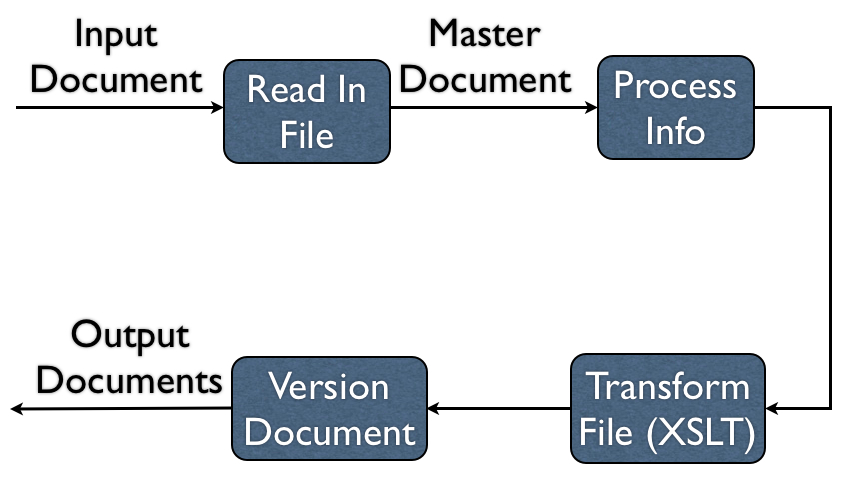
\includegraphics[width=.90\textwidth]{images/software_workflow}
			\caption[Software Workflow]{Example software workflow to be used throughout this report}
			\label{fig:software_workflow}
		\end{figure}\\
		\begin{figure}[htp]
			\centering
			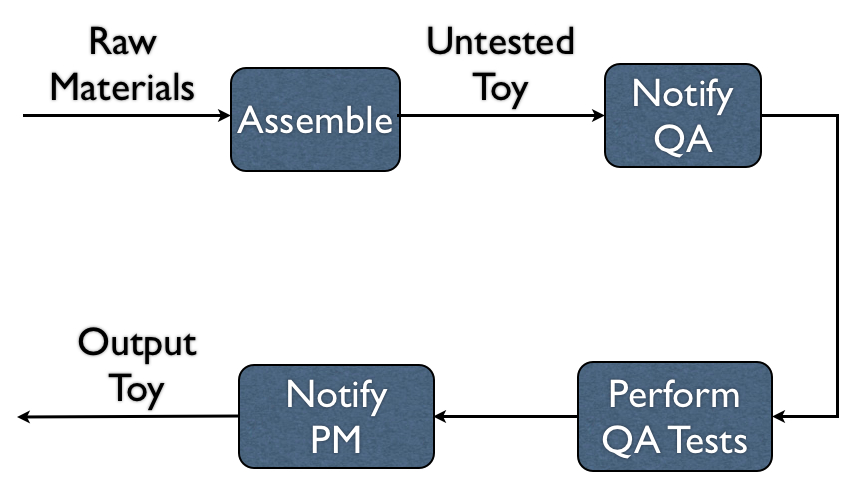
\includegraphics[width=.90\textwidth]{images/physical_workflow}
			\caption[Physical Workflow]{Example physical workflow to be used throughout this report}
			\label{fig:physical_workflow}
		\end{figure}\\
In addition, this report will further narrow the scope down to only addressing the significance of Continuous Integration on large projects. A large project is defined as a project where many teammates work together to complete a task, whereas a small project would have less than four people working on the task.  This is due to the fact that these concepts have greater benefits for larger projects and it is easier to see these benefits if applied to a larger project. However, all these concepts may also be applied and scaled down for smaller projects should the reader require.  Smaller projects still benefit greatly from these concepts, it is just easier to see the benefits in a larger project.  Thus any reference to the ``project'' refers to a large project.
	% subsection scope (end)

	\subsection{Outline} % (fold)
	\label{sub:outline}
There are two sections in this report that analyze key concepts that pertain to workflow automation and an analysis of the the advantages and disadvantages that applying these key concepts will bring. Throughout the report, a variety of terms are used so a glossary of terms has been included for reference. The first section of the report introduces a selection of key concepts of Continuous Integration and gives an analysis of how these concepts would be applied to workflow automation.  These key concepts include ``Maintain a Single Source Repository'', ``Make Your Build Self-Testing'', and ``Keep you Build Fast''.  The second section of this report gives a brief analysis of the benefits of automation and analyzes the advantages and disadvantages of applying these concepts for automation based on two factors: efficiency and resources required.
	% subsection outline (end)

% section introduction (end)
